%%%%%%%%%%%%%%%%%%%%%%%%%%%%%%%%%%%%%%%%%%%%%%
%% Copyright 2020 Andrew Cuccinello
%%
%% Licensed under the Apache License, Version 2.0 (the "License");
%% you may not use this file except in compliance with the License.
%% You may obtain a copy of the License at
%%
%%     http://www.apache.org/licenses/LICENSE-2.0
%%
%% Unless required by applicable law or agreed to in writing, software
%% distributed under the License is distributed on an "AS IS" BASIS,
%% WITHOUT WARRANTIES OR CONDITIONS OF ANY KIND, either express or implied.
%% See the License for the specific language governing permissions and
%% limitations under the License.

\documentclass{article}
\usepackage{fullpage}
\usepackage{graphicx}
\usepackage{hyperref}
\hypersetup{
colorlinks=true,
linkcolor=blue,
filecolor=magenta,
urlcolor=cyan,
}

\title{%
PDFoundry \\
\large User Manual\\
For v0.7.X}
\date{}
\author{}

\setcounter{tocdepth}{2}
\begin{document}
    \begin{figure}[t]
        \centering
        
\includegraphics[width=0.5\textwidth]{images/fvtt-d20.png}
    \end{figure}
    \maketitle

    If you're seeing this - it means your system now supports \textit{PDFoundry}, a FoundryVTT PDF reader. This guide goes over the features available and their use. This user manual also functions as a demo, and you can always access it through the \textbf{settings menu}, if you wish to do so later.

    \tableofcontents

    \section{Creating \& Opening PDFs}
    \label{sec:creating-opening-pdfs}

    Once you've installed PDFoundry, you're almost ready to view a PDF - the only thing you'll have to do is tell PDFoundry where to find it, and what type of PDF it should be opened as.

    \subsection{Adding a PDF}
    This section outlines basic steps required to adding a new PDF and outlines what each PDF setting does.

    \begin{description}
        \item [Step 1] Open the \textbf{Journal Entries} and click \textbf{Create PDF}. Enter a \textbf{Name}, in Figure~\ref{new-item} I've chosen to add the core rule book for the RPG \textit{Lancer} (\href{https://massif-press.itch.io/corebook-pdf-free}{available for free online!}), so I'll name this one \textit{Lancer Core Rulebook}. Select \textbf{PDFoundry\_PDF} for the \textbf{Type} drop-down, then click \textbf{Create Item}.

        % \begin{figure}[h]
        %     \centering
        %     \begin{minipage}[t]{0.45\textwidth}
        %         \centering
        %         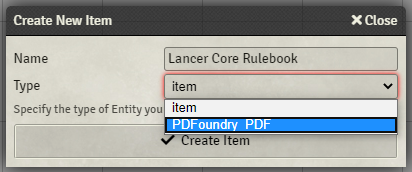
\includegraphics[width=\textwidth]{images/new-item.png}
        %         \caption{A created item in the \textbf{Item Directory}}
        %         \label{new-item}
        %     \end{minipage}
        %     \hfill
        %     \begin{minipage}[t]{0.45\textwidth}
        %         \centering
        %         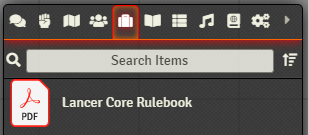
\includegraphics[width=\textwidth]{images/new-item-created.png}
        %         \caption{The \textbf{New Item} dialog}
        %         \label{new-item-created}
        %     \end{minipage}
        % \end{figure}

        \item [Step 2] After you've hit \textbf{Create PDF} the \textbf{PDF Config} should open automatically and look something like Figure~\ref{fig:new-pdf-config}. You'll also see the PDF get placed in your \textbf{Journal Entries}, as in Figure~\ref{fig:new-pdf-sidebar}. There are a bunch of fields on the \textbf{PDF Config}, \textit{PDF Name} is already filled in for us (but we can change it if we want!). Next let's fill in all the fields.

        \begin{figure}[h]
            \centering
            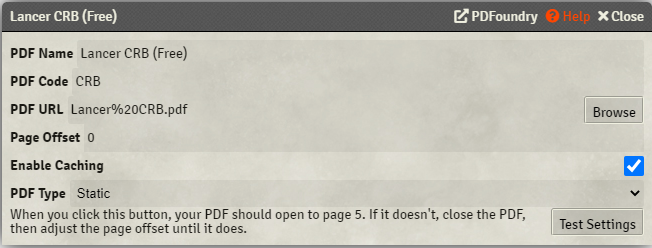
\includegraphics[width=1\textwidth]{images/new-pdf-config.png}
            \caption{The \textbf{PDF Config}}
            \label{fig:new-pdf-config}
        \end{figure}

        \item [\textit{PDF Code}] This is a short (usually five characters or less, but as many as you want) identifier you will use in most systems. Systems with support for PDFoundry (or modules that add support for PDFoundry to a system) may make use of this as a short-hand to open PDFs or display links.

        \item [\textit{PDF URL}] This is the path to the PDF on your server. The browse button will allow you to select or upload a PDF from your computer, or choose a PDF from a S3 bucket.

        \item [\textit{Page Offset}] Some PDF files have extra pages before the first page, such as a title or an unnumbered index page. You can use this to synchronize the PDF page to the book page. The Lancer book doesn't need an offset, so it's zero here.

        \item [\textit{Enable Caching}] Tick this box to enable caching for this PDF. Caching will help PDFs load \textit{significantly} faster after the first time they are loaded by preserving a copy locally on the user's computer. \underline{To preload PDFs, this must be enabled.}

        \item [\textit{PDF Type}] PDFoundry supports three types of PDFs - \textbf{Static} PDFs, \textbf{Form Fillable (Unlinked)} PDFs, and \textbf{Form Fillable (Actor Sheet)} PDFs. If you don't want any interactive elements like you may find in some character sheets, select \textbf{Static} for now. The difference between \textbf{Form Fillable (Unlinked)} PDFs and \textbf{Form Fillable (Actor Sheet)} PDFs is explained in Section~\ref{sec:form-fillable-pdfs}.

        \item [Step 3] Now that we've entered all our settings in, we can use the \textbf{Test Settings} button to open the PDF to page 5. We want the PDF to open to page 5 of the book, so that when we have a page reference it opens to the correct page. Play around with the offset until the viewer opens the PDF to the correct pages.

    \end{description}

    That's it, we've added a new PDF!

    \subsection{Context Menu}
    We saw the PDF appear in the \textbf{Journal Entries} earlier, when we \hyperref[sec:creating-opening-pdfs]{created a new PDF}. Figure~\ref{fig:new-pdf-sidebar} shows the context menu options for PDF items, and highlights two import elements. You can open the context menu with \textbf{right click}. There are a bunch of options that you as the GM can see, while players will only be able to see the \textbf{Open PDF} option, provided they have permissions of at least \textbf{Observer}.

    \begin{figure}[h]
        \centering
        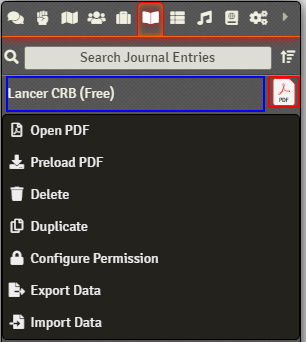
\includegraphics[width=0.5\textwidth]{images/new-pdf-sidebar.png}
        \caption{The PDF \textbf{Sidebar \& Context Menu}}
        \label{fig:new-pdf-sidebar}
    \end{figure}

    \textbf{Left Clicking} the \textbf{blue} area will open the \hyperref[sec:creating-opening-pdfs]{PDF Config} window. \textbf{Right Clicking} it will open the context menu. \textbf{Left Clicking} the \textbf{red} PDF thumbnail will open the PDF to the first page, which can save you a click.

    \begin{description}

        \item [Open PDF] (All Users) This one should be mostly self explanatory. It won't show up unless the \textbf{PDF URL} has been fully configured in the \hyperref[sec:creating-opening-pdfs]{PDF Config} window. Clicking on it opens the PDF to the very first page. Note that you can't open \textbf{Form Fillable (Actor Sheet)} PDFs this way, they have to be opened with the actor.

        \item [Preload PDF] (GM Only) Click on it will immediately cache the PDF on all \underline{connected} users' computers. This may be advantageous in cases where you expect to often use a single large book and don't want users downloading the PDF files to interrupt other goings on in the game.

        \item [Delete] (GM Only) This will irrevocably delete the link to the PDF file. The PDF file itself is not affected.

        \item [Duplicate] (GM Only) This will duplicate the link to the PDF file by creating a copy of the journal entry.

        \item [Configure Permission] (GM Only) This will allow you to grant visibility of the PDF to players, either individually or all players. The permissions work much like permissions for other things in Foundry; however, if the PDF is visible to the player at all (that is if their permissions are anything \underline{except 'None'}) the user will be able to right click on the PDF to open it, and any other links to the PDF will function correctly (such as 'open to page' links added by a system).

        \item [Export Data] (GM Only) This will allow you to export a file that can later be used with the \textbf{Import Data} option.

        \item [Import Data] (GM Only) This will allow you to import the settings for a PDF (Name, Code, URL, etc) from a file created with the \textbf{Export Data} option.

    \end{description}

    \section{Rich PDF Links in Journals \& Editors}

    Once we've added a PDF to Foundry, it can be embedded in journals and other rich text editor areas added by systems in items, actors, and more. You can quickly create a PDF link by dragging and dropping a PDF item from the \textbf{Journal Entries}, which will create a link to the first page of the PDF. You can then adjust the page to a page of your choosing.

    The format for a rich text link in a Journal or Item Sheet is as follows.

    \begin{verbatim}
        @PDF[Core Rulebook|page=135]{Combat: Grappling & Shoving}
              PDF Source     Page             Link Text
    \end{verbatim}

    \begin{figure}[h]
        \centering
        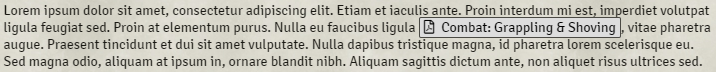
\includegraphics[width=1\textwidth]{images/rich-text-link-example.png}
        \caption{The PDF journal link created from the above example.}
        \label{rich-text-link-example}
    \end{figure}

    \begin{description}

        \item [PDF Source] This specifies which PDF should be opened, and can be either a \textbf{PDF Name} or \textbf{PDF Code}.

        \item [Page] (Optional) This specifies which page should be opened. You can omit this option and the PDF will be opened to the first page. If you were to omit the page from the example above, the example would be changed to look like this, and would open the "Core Rulebook" to the first page.

        \begin{verbatim}
        @PDF[Core Rulebook]{Combat: Grappling & Shoving}
              PDF Source             Link Text
        \end{verbatim}

        \item [Link Text] The link text field specifies what text should be displayed. It supports rich text, so you can have bold links, underlined links, header links, and more. Unicode characters and emoji are also supported.

    \end{description}

    \subsection{Permissions}
    A quick note on permissions - PDF links in journals will only be displayed to those with the ability to see the PDF in the \textbf{Journal Entries}. If a player is unable to see the PDF, they will instead see the link text by itself and no link will be rendered. An example of what this looks like is shown in Figure~\ref{fig:rich-text-link-example-permissions}.

    \begin{figure}[h]
        \centering
        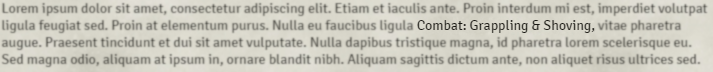
\includegraphics[width=1\textwidth]{images/rich-text-link-example-permissions.png}
        \caption{The PDF journal link created from the above example as seen by a player who cannot view the specified PDF.}
        \label{fig:rich-text-link-example-permissions}
    \end{figure}

    \section{Form Fillable PDFs}
    \label{sec:form-fillable-pdfs}

    Support for Form Fillable PDFs is the largest and most ambitious feature that PDFoundry supports. You can almost entirely make use of existing PDF character sheets, inventory trackers, and more.

    Please note that 'JavaScript' areas are not supported at the moment, so currently you cannot set up automation.

    Two types of Form Fillable PDFs are available - \textbf{Form Fillable (Unlinked)} PDFs and \textbf{Form Fillable (Actor Sheet)} PDFs.

    \subsection{Form Fillable (Unlinked) PDFs}
    Unlinked PDFs contain form fillable elements and save the data contained within those elements. However, they save the data once per PDF. That is, all users who view the PDF will see the same data, and changes will be synchronized between all viewing users, but there is no way to link the data with an actor or instance it in any way. This type of PDF is useful for party inventory sheets, board game sheets, and any other type of PDF where you want only a single copy of the data on the PDF.

    \subsection{Form Fillable (Actor Sheet) PDFs}
    This is the more complex but potentially more useful type of form fillable PDF. It allows you to use a form fillable PDF to act as an actor sheet! PDFoundry is even capable of synchronizing the data with the game world in real time, so with a little bit of effort, you can edit a form fillable PDF so it reflects changes to an actors HP or have it display system specific information.

    \subsubsection{Linking an Actor}
    Once you've created a \textbf{Form Fillable (Actor Sheet)} as outlined in the \hyperref[sec:creating-opening-pdfs]{section on creating a new PDF}, open the actor you wish to use the sheet for and click the \textbf{Sheet} button on the title bar as shown in Figure~\ref{fig:actor-sheet-header}. After, select "pdfoundry.PDFActorSheetAdapter" from the drop-down as shown in Figure~\ref{fig:actor-sheet-select}. The top drop-down will let you select the sheet for an individual actor, while if you wish to use PDFoundry for all actors, select it for the bottom drop-down as well.

    \begin{figure}[h]
        \centering
        
\includegraphics[width=1\textwidth]{images/actor-sheet-header.png}
        \caption{Select the Sheet here.}
        \label{fig:actor-sheet-header}
    \end{figure}

    \begin{figure}[h]
        \centering
        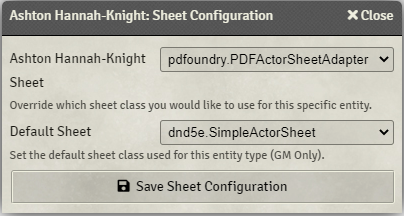
\includegraphics[width=0.5\textwidth]{images/actor-sheet-select.png}
        \caption{Foundry VTT Sheet Configuration}
        \label{fig:actor-sheet-select}
    \end{figure}

    You'll see a blank sheet should come up. The header for this sheet should look pretty similar to the header from the last one. This time you'll notice two new buttons \textbf{Inspect Data} and \textbf{Sheet Select}.

    \begin{figure}[h]
        \centering
        
\includegraphics[width=1\textwidth]{images/actor-sheet-viewer-header.png}
        \caption{The PDFoundry Actor Sheet Header}
        \label{fig:actor-sheet-header}
    \end{figure}

    \begin{description}

        \item [Sheet Select] (Red, GM Only) This will allow us to tell PDFoundry which of the configured PDF sheets should be used to display this actor. You'll want to set a sheet for PDFoundry to use when you first set the actor to be opened by PDFoundry, otherwise it will open to a blank viewer.

        \item [Inspect Data] (Blue, GM Only) Will allow us to see data paths PDFoundry will recognize and their current values. For more of an explanation, see \hyperref[sec:data-paths]{Section \ref{sec:data-paths}: Data Paths}.

    \end{description}

    \section{Data Paths}
    \label{sec:data-paths}

    Finally there's the Inspect Data button found at the top of PDFoundry actor sheets, which will give you the special names (called data paths) that may be used for the fields that will be synchronized with Foundry. These are system specific, and their value is listed next to them so you can play around and find which you are looking for.

    For example, if you want to set up a character sheet with the "Simple Worldbuilding" system to reflect changes to current and maximum hit points, you can use the data paths "data.health.value" and "data.health.max" for current and maximum hit points respectively. You use the name attribute when you edit the PDF in Acrobat (or whatever other editor you use). So, to reiterate - a value of data.health.value would synchronize the field's value with the actor's current hit points only in the "Simple Worldbuilding" system. Again, see the Inspect Data window for system-specific paths.

    \begin{figure}[h]
        \centering
        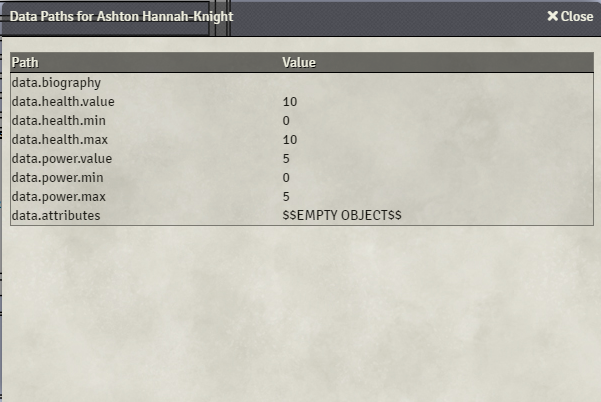
\includegraphics[width=1\textwidth]{images/actor-sheet-inspect-data.png}
        \caption{The \textbf{Inspect Data} Window}
        \label{fig:actor-sheet-inspect-data}
    \end{figure}

    Note these paths are only viewable when data currently exists there, so you may see them appear and disappear as you make edits to the actor with a normal actor sheet if the system does not place some value there by default - this may or may not be improved in the future.

    Note that any other data path will work (so you could set the name attribute of a field to "FooBar", and it would save and load just fine), but will only the special data paths visible in the Inspect Data window will be synchronized for use in the game world natively (without some programming knowledge, at least). That means you can use a form fillable sheet as-is, but with a little work you can make it pretty dynamic. The only other special data path that is available at the moment is name, which is used for the actor's name (so you would set the name attribute of the field to the value name when you edit the PDF in Acrobat).

    Note there will likely be improvements to this helper window in the future.

    \section{Settings}
    There two settings at present for PDFoundry. They are located with your system settings in the \textbf{Game Settings} $>$ \textbf{Configure Settings} $>$ \textbf{System Settings} menu.

    \begin{description}

        \item \subsection{PDF Cache Size} This allows individual users to set how much hard drive space should be allowed to be taken up by the PDF cache. When this amount is exceeded, PDFoundry will prune existing cached PDF files in reverse order of most recently accessed. That is to say, PDF files will be removed from the cache starting with the file that has least recently accessed.

        \item \subsection{Show Shared PDFs in Existing Viewer} With this setting enabled, when a user opens a PDF for you with the 'Show to...' button on the top of the PDF viewer, the PDF will open in your existing viewer if you are already looking at the PDF.

    \end{description}

\end{document}